\section{优化问题的表述}
\label{sec:opt-formulation}

我们先要把“选最好的”这句话写到可以判断对错的程度。为此要说清在哪些候选里选、按什么标准比较，以及“选出来”究竟指什么。我们先看两个具体任务，再抽出共同的写法。

\paragraph{资源分配}
一个车间生产两种产品，产量分别记为$x_1,x_2$，单位是批。每批产品一的利润是$3$，产品二的利润是$2$。每批产品各用$1$个工时，每天共有$4$个工时；每批产品一用$2$份原料，产品二用$1$份，每天共有$6$份原料。产量不能为负。

车间能调整的只有$x_1,x_2$这两个数，把它们合成向量$\bm{x}=(x_1,x_2)^\top\in\mathbb{R}^2$。要比较的是利润$3x_1+2x_2$。允许的产量组合满足
\begin{equation}
 x_1+x_2\leq4,\qquad 2x_1+x_2\leq6,\qquad x_1\geq0,\qquad x_2\geq0.
 \label{eq:opt-resource-constraints}
\end{equation}

这里要的是利润最大，而全卷统一讨论最小化。两者只差一个符号：最大化$3x_1+2x_2$与最小化$-(3x_1+2x_2)$选出的产量相同，最大利润等于最小值的相反数。于是取
\begin{equation}
 f(\bm{x})=-(3x_1+2x_2).
 \label{eq:opt-resource-objective}
\end{equation}

把约束~\eqref{eq:opt-resource-constraints}画在平面上，四条直线围出图~\ref{fig:opt-resource-region}中的浅蓝色四边形，产量只能在其中选。虚线是利润相等的产量组合，线旁的数字是利润值，线越往右上利润越高。利润为$10$的线恰好擦过四边形的一个角$(2,2)$，再往外推，线上就没有允许的点了。

\begin{BookInlineFigure}
  \centering
  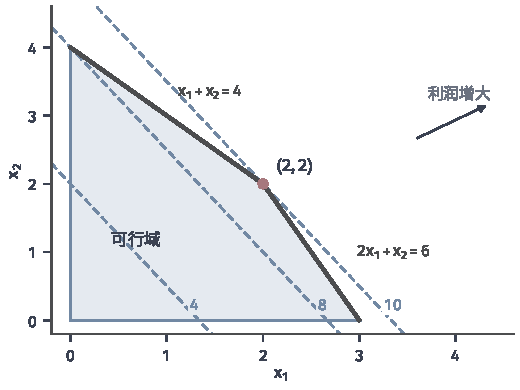
\includegraphics[width=88mm]{figures/05-optimization/01-linear-programming/matplotlib/opt-resource-region/figure.pdf}
  \caption{资源分配问题。浅蓝色四边形是全部允许的产量组合，顶点为$(0,0),(3,0),(2,2),(0,4)$；深灰粗线是工时约束与原料约束的边界。蓝色虚线是利润等于$4,8,10$的直线，红点$(2,2)$是利润为$10$的线与四边形唯一的公共点。}
  \label{fig:opt-resource-region}
\end{BookInlineFigure}

\paragraph{二次拟合}
第二个任务来自数据。设有$N$个观测和$n$个待定系数，矩阵$\bm{A}\in\mathbb{R}^{N\times n}$的第$i$行记录第$i$个观测的输入，向量$\bm{b}\in\mathbb{R}^N$记录观测值。系数$\bm{x}\in\mathbb{R}^n$给出的预测是$\bm{A}\bm{x}$，我们用平方误差比较不同的系数：
\begin{equation}
 f(\bm{x})=\frac12\lVert\bm{A}\bm{x}-\bm{b}\rVert_2^2+\frac{\gamma}{2}\lVert\bm{x}\rVert_2^2,\qquad\gamma\geq0.
 \label{eq:opt-ridge}
\end{equation}
第一项衡量预测与观测的差距，第二项称为正则项，系数$\gamma$决定对大系数收多少“费”。这个目标是$\bm{x}$的二次函数，所以称为二次拟合。

全章反复使用一个最小的实例：只有一个观测，$N=1$；两个系数，$n=2$；$\bm{A}=(1\ \ 1)$，$\bm{b}=2$。它的含义是“只测到两个量的和约等于$2$”。此时
\begin{equation}
 f(\bm{x})=\frac12(x_1+x_2-2)^2+\frac{\gamma}{2}(x_1^2+x_2^2).
 \label{eq:opt-ridge-instance}
\end{equation}
这个例子小到可以手算，却已经包含解不唯一、平坦方向和误差指标互相矛盾这些现象。

\paragraph{统一的写法}
两个任务都是在一个集合里选$\bm{x}$，使一个数尽量小。我们把这个结构固定下来，并同时规定全卷的记号。

\begin{definition}[优化问题]
\label{def:opt-problem}
给定集合$\bm{C}\subseteq\mathbb{R}^n$与函数$f:\bm{C}\to\mathbb{R}$，寻找使$f$尽量小的$\bm{x}\in\bm{C}$的任务称为\term{优化问题}（optimization problem），写作
\begin{equation}
 \min_{\bm{x}\in\bm{C}}f(\bm{x}).
 \label{eq:opt-general}
\end{equation}
$\bm{x}$称为\term{决策变量}（decision variable），$f$称为\term{目标函数}（objective function），$\bm{C}$称为\term{可行集}（feasible set），$\bm{C}$中的点称为\term{可行点}（feasible point）。
\end{definition}

可行集常常由一组条件给出。全卷把不等式都整理成“$\leq0$”的形式，写作
\begin{equation}
 \bm{C}=\bigl\{\bm{x}\in\mathbb{R}^n:\ g_i(\bm{x})\leq0,\ i=1,\ldots,m;\ h_j(\bm{x})=0,\ j=1,\ldots,p\bigr\}.
 \label{eq:opt-constraint-form}
\end{equation}
其中$g_i$是不等式约束，共$m$个；$h_j$是等式约束，共$p$个。资源分配里没有等式约束，四个不等式约束是
\[
 g_1(\bm{x})=x_1+x_2-4,\quad g_2(\bm{x})=2x_1+x_2-6,\quad g_3(\bm{x})=-x_1,\quad g_4(\bm{x})=-x_2.
\]
二次拟合里没有约束，$\bm{C}=\mathbb{R}^n$。

$\bm{C}$与$f$必须一起给定，问题才算确定。对二次拟合而言，改变$\gamma$是在改变候选之间的比较标准，全部候选都还在；加上硬性要求$x_1\geq1.2$则是把一部分候选直接淘汰。前者像调整评分表，后者像修改参赛资格。两种改动都可能让答案变化，但机制不同，这一区别到本节末尾还会出现。

\paragraph{最优值与最优解}
“最低点”其实包含两个问题：最低的高度是多少，这个高度在哪里取得。前者是一个数，后者是一个位置。两者要分开定义，因为第一个问题有答案时，第二个问题可能没有。

\begin{definition}[最优值与最优解]
\label{def:opt-optimal-value}
问题~\eqref{eq:opt-general}的\term{最优值}（optimal value）是
\begin{equation}
 f^\star=\inf_{\bm{x}\in\bm{C}}f(\bm{x})\in[-\infty,+\infty],
 \label{eq:opt-optimal-value}
\end{equation}
并约定空集上的下确界为$+\infty$。若可行点$\bm{x}^\star$满足$f(\bm{x}^\star)=f^\star$，就称它为\term{最优解}（optimal solution）。全体最优解组成的集合记为$\argmin_{\bm{x}\in\bm{C}}f(\bm{x})$。这个集合非空时，称最优值被达到。
\end{definition}

符号$\min$在式~\eqref{eq:opt-general}中只表示提出任务。若有人写“最小值等于某个数”，他同时断言了这个数被某个可行点取得；若只知道下确界，应当写$\inf$。

现在解资源分配问题。要证明$(2,2)$最好，需要两件事：所有可行点的利润都不超过某个数，并且$(2,2)$达到了这个数。第一件事可以这样做：利润系数$(3,2)$恰好是两条资源约束系数$(1,1)$与$(2,1)$之和，所以对任意可行点，把两条约束相加，得到
\[
 3x_1+2x_2=(x_1+x_2)+(2x_1+x_2)\leq4+6=10.
\]

这说明$f(\bm{x})\geq-10$对所有可行点成立。等号成立当且仅当两条资源约束同时取等号，也就是
\[
 x_1+x_2=4,\qquad 2x_1+x_2=6.
\]
解得$\bm{x}=(2,2)$，它满足非负约束，因而可行。于是
\[
 f^\star=-10,\qquad \argmin_{\bm{x}\in\bm{C}}f(\bm{x})=\{(2,2)\}.
\]

这个论证的结构值得记住：一个对所有可行点成立的下界，加上一个达到该下界的可行点，从两侧把最优值夹住，两者缺一不可。只有下界，不知道它是否够紧；只有候选点，不知道还有没有更好的。第~\ref{chap:linear-programming}章会说明，“给约束配权重再相加”可以系统地做。

二次拟合实例~\eqref{eq:opt-ridge-instance}取$\gamma=0$时，$f(\bm{x})=\frac12(x_1+x_2-2)^2\geq0$。凡满足$x_1+x_2=2$的点都使$f=0$，所以$f^\star=0$，最优解是一整条直线。比如$(1,1)$和$(3,-1)$都最优。数据只约束了两个量的和，没有约束它们的差，参数不唯一并不是计算失败，而是问题本身没有提供区分它们的信息。

\paragraph{三种没有最优解的情形}
并不是每个问题都有解，失败有三种不同的方式，分别出在不同的环节。

\begin{itemize}
 \item \term{不可行}（infeasible）：$\bm{C}=\varnothing$，此时$f^\star=+\infty$。例如同时要求$x\leq0$与$x\geq1$。
 \item \term{无下界}（unbounded below）：$\bm{C}\neq\varnothing$且$f^\star=-\infty$。例如在$\mathbb{R}$上最小化$f(x)=x$，取$x=-k$可得$f=-k\to-\infty$。
 \item 下确界未达到：$f^\star$是有限实数，但$\argmin$为空。例如在$\mathbb{R}$上最小化$f(x)=e^x$。
\end{itemize}

第三种最容易被忽略。对$e^x$，处处有$e^x>0$，又有$e^{-k}\to0$，所以$f^\star=0$；但没有$x$使$e^x=0$。只报告“最优值是$0$”而不说明它未被达到，读者会以为存在一个最优的$x$。图~\ref{fig:opt-failure-modes}把三种情形放在一起。

\begin{BookInlineFigure}
  \centering
  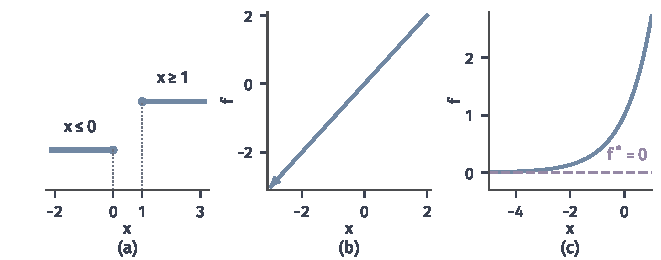
\includegraphics[width=112mm]{figures/05-optimization/01-linear-programming/matplotlib/opt-failure-modes/figure.pdf}
  \caption{优化问题没有最优解的三种方式。(a)约束$x\leq0$与$x\geq1$对应的两段蓝色射线没有公共点，可行集为空。(b)$f(x)=x$沿箭头方向无限下降，最优值为$-\infty$。(c)$f(x)=e^x$趋于紫色虚线$f^\star=0$却永远碰不到：最优值有限，但没有点取得它。}
  \label{fig:opt-failure-modes}
\end{BookInlineFigure}

\paragraph{局部最优与全局最优}
前面的最优解要和所有可行点比。实际计算时，我们往往只看得见当前点附近的情况，所以还需要一个只和附近比较的概念。“附近”用开球表示：
\[
 \bm{B}(\bm{x},r)=\{\bm{y}:\lVert\bm{y}-\bm{x}\rVert_2<r\}.
\]

\begin{definition}[局部最优解]
\label{def:opt-local}
设$\bm{x}^\star\in\bm{C}$。若存在$r>0$，使
\begin{equation}
 f(\bm{x}^\star)\leq f(\bm{x})\qquad\text{对所有}\ \bm{x}\in\bm{C}\cap\bm{B}(\bm{x}^\star,r)\ \text{成立},
 \label{eq:opt-local}
\end{equation}
就称$\bm{x}^\star$为\term{局部最优解}（local minimizer）。若对其中所有$\bm{x}\neq\bm{x}^\star$都有严格不等式，就称它为\term{严格局部最优解}（strict local minimizer）。定义~\ref{def:opt-optimal-value}中的最优解也称\term{全局最优解}（global minimizer）。
\end{definition}

比较的范围是$\bm{C}\cap\bm{B}(\bm{x}^\star,r)$，不是整个球。可行集边界上的点只需要和球内的可行点比较，球里伸出可行集的部分不参加比较。下面的例子同时展示洼地与边界。

\begin{example}[两个洼地与一个边界]
\label{ex:opt-local-global}
在可行集$\bm{C}=[-1.5,1.5]$上最小化
\[
 f(x)=\frac{x^4}{4}-\frac{x^3}{3}-x^2.
\]
先求导并分解因式：
\[
 f'(x)=x^3-x^2-2x=x(x-2)(x+1).
\]
所以$f'$在$x=-1,0,2$处为零。其中$x=2$在可行集之外。由$f'$的符号，$f$在$[-1.5,-1]$上递减，在$[-1,0]$上递增，在$[0,1.5]$上递减。

因此$x=-1$附近的可行点函数值都不低于$f(-1)$，它是局部最优解。$\bm{C}$上的最小值只可能出现在$x=-1$或右端点$x=1.5$，两处的函数值是
\[
 f(-1)=-\frac{5}{12}\approx-0.417,\qquad f(1.5)\approx-2.109.
\]
所以全局最优解是$x=1.5$。这一点在边界上，那里$f'(1.5)=-1.875\neq0$：函数还在向右下降，只是可行集不允许再往右走。
\end{example}

图~\ref{fig:opt-local-global}画出这个例子，地形的比喻在这里很贴切。黄点是一个洼地的底部，站在那里四周都更高，它却不是最低处。红点是真正的最低处，脚下的地面还是斜的，挡住我们的是边界，不是地形。可行集右侧还有更低的点$x=2$，但它不是候选，与问题无关。

\begin{BookInlineFigure}
  \centering
  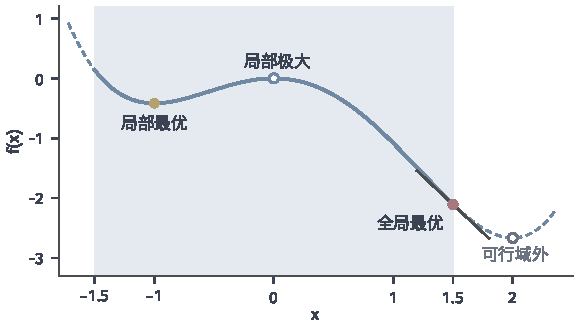
\includegraphics[width=98mm]{figures/05-optimization/01-linear-programming/matplotlib/opt-local-global/figure.pdf}
  \caption{$f(x)=x^4/4-x^3/3-x^2$在$\bm{C}=[-1.5,1.5]$（浅蓝色带）上的局部与全局最优。蓝色实线是$\bm{C}$上的图像，虚线是$\bm{C}$外的部分。黄点$x=-1$是局部最优解，红点$x=1.5$是全局最优解，该处的短切线不水平，斜率为$-1.875$。空心点分别是局部极大点$x=0$和可行集外的$x=2$。}
  \label{fig:opt-local-global}
\end{BookInlineFigure}

严格局部最优只说明一个小邻域内没有并列者，并不排除远处有同样低的点。函数$(x^2-1)^2$在$x=\pm1$处都取到全局最小值$0$，两点各自是严格局部最优解，全局最优解却有两个。

\paragraph{把约束并入目标}
到目前为止，可行集和目标是两个分开的对象。后面常要把几种代价相加，或者用同一个工具处理各种约束，分开写很不方便。一个自然的想法是：给不可行的点一个大到不可能被选中的值。任何有限的数都不够保险，所以我们允许函数取$+\infty$。

\begin{definition}[扩展实值函数与约束指标函数]
\label{def:opt-extended}
取值于$\mathbb{R}\cup\{+\infty\}$的函数称为\term{扩展实值函数}（extended real-valued function）。它的\term{有效定义域}（effective domain）是$\operatorname{dom}F=\{\bm{x}:F(\bm{x})<+\infty\}$；有效定义域非空时，称$F$为\term{适当函数}（proper function）。集合$\bm{C}\subseteq\mathbb{R}^n$的\term{约束指标函数}（constraint indicator function）是
\begin{equation}
 \iota_{\bm{C}}(\bm{x})=\begin{cases}0,&\bm{x}\in\bm{C},\\+\infty,&\bm{x}\notin\bm{C}.\end{cases}
 \label{eq:opt-constraint-indicator}
\end{equation}
扩展实值目标$F$的最优解集合规定为
\begin{equation}
 \argmin F=\{\bm{x}\in\operatorname{dom}F:F(\bm{x})=\inf F\}.
 \label{eq:opt-extended-argmin}
\end{equation}
\end{definition}

对可行集$\bm{C}$非空的问题，令$F=f+\iota_{\bm{C}}$，也就是在$\bm{C}$上$F=f$，在$\bm{C}$外$F=+\infty$。这里$f+\iota_{\bm{C}}$在$\bm{C}$外按$+\infty$理解，不要求$f$在那里有定义。逐项核对这种写法保留了什么。

首先，$\operatorname{dom}F=\bm{C}$，所以取有限值的候选恰好是可行点。其次，$F$与$f$在可行点上取值相同，其余点取$+\infty$，不影响下确界，于是
\[
 \inf_{\mathbb{R}^n}F=\inf_{\bm{x}\in\bm{C}}f(\bm{x}).
\]
最后，最优解只在$\operatorname{dom}F=\bm{C}$中找，所以$\argmin F$与原问题的最优解集合相同。若$\bm{C}=\varnothing$，则$F\equiv+\infty$不是适当函数，应报告不可行；定义中限定在$\operatorname{dom}F$内找解，正是为了避免说成“每一点都最优”。

\paragraph{约束指标函数不是普通指示函数}
名称相近的普通\term{指示函数}（indicator function）$\mathbb{1}_{\bm{C}}$在$\bm{C}$上取$1$，在$\bm{C}$外取$0$。两者的取值表放在一起，就能看出差别。

\begin{BookInlineTable}
  \centering
  \begin{tabular}{@{}lcc@{}}
    \toprule
     & $\bm{x}\in\bm{C}$ & $\bm{x}\notin\bm{C}$\\
    \midrule
    约束指标函数$\iota_{\bm{C}}$ & $0$ & $+\infty$\\
    普通指示函数$\mathbb{1}_{\bm{C}}$ & $1$ & $0$\\
    \bottomrule
  \end{tabular}
  \caption{约束指标函数与普通指示函数的取值。前者用于把违规点排除，后者只是记录一个点是否属于集合。}
  \label{tab:opt-indicators}
\end{BookInlineTable}

两者的方向也相反：$\iota_{\bm{C}}$在集合内为小值，$\mathbb{1}_{\bm{C}}$在集合内为大值。用一个例子看把它们加到目标上的后果。在约束$x\leq1$下最小化$(x-2)^2$，可行集记为$C=(-\infty,1]$。这个问题的最优解是$x=1$，最优值为$1$。

图~\ref{fig:opt-extended-value}比较三种加法。加$\iota_C$得到的问题就是原问题。加$\mathbb{1}_C$则让可行点反而贵了$1$，最小点跑到$x=2$，违反约束。

第三种是有限惩罚，它按违规程度收费。改为最小化$(x-2)^2+\max\{0,x-1\}$，在$x>1$的范围内令导数为零：
\[
 2(x-2)+1=0,\qquad x=1.5.
\]
此处函数值是$0.25+0.5=0.75$，低于约束问题的最优值$1$，所以惩罚问题的最小点违反了约束。

\begin{BookInlineFigure}
  \centering
  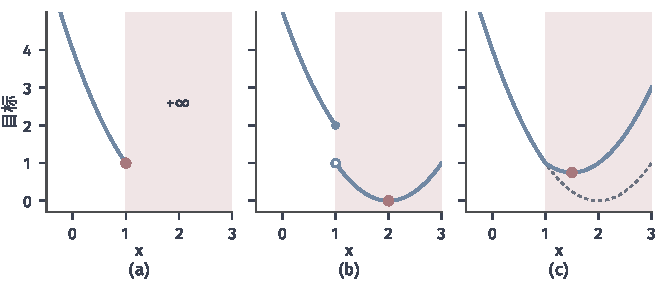
\includegraphics[width=112mm]{figures/05-optimization/01-linear-programming/matplotlib/opt-extended-value/figure.pdf}
  \caption{把约束$x\leq1$并入目标$(x-2)^2$的三种做法，浅红区域是不可行的点，红点是所得问题的最小点。(a)加约束指标函数，浅红区域取$+\infty$，最小点$x=1$与原问题相同。(b)加普通指示函数，可行点上升$1$，最小点变成不可行的$x=2$。(c)加有限惩罚$\max\{0,x-1\}$（灰色点线是原目标），最小点$x=1.5$仍不可行。}
  \label{fig:opt-extended-value}
\end{BookInlineFigure}

约束指标函数只是把同一个问题换了写法；有限惩罚改变了问题，只是不喜欢违规，并不禁止违规。惩罚要多大才能恢复约束，是第~\ref{chap:penalty-multiplier-methods}章的话题。今后需要时，我们把约束问题~\eqref{eq:opt-general}直接写成扩展实值目标的最小化，两种写法描述同一个问题。
